%% ===========================================================================
\section{Findings}
\budget{3,000}

\subsection{Crisis type, not era, fixes the compositional signature (R1)}
\budget{425}

\begin{description}
\item[Claim.] The Frame $\times$ Sentiment signature is a property of crisis
  \emph{type}; six years of platform change do not move it.

\item[Primary evidence.] Pairwise cosine between 18-dim event signatures,
  thread-clustered bootstrap. Pulwama $\leftrightarrow$ Sindoor \textbf{0.0074}
  [0.0022, 0.0313]; Article 370 $\leftrightarrow$ Sindoor 0.2749 [0.2332,
  0.3114]. \textbf{Separation is CI-based and contrast-specific}: across the 6
  military--military pairs, max CI hi $=\textbf{0.0768}$; across the 4
  military--constitutional pairs, min CI lo $=\textbf{0.1359}$; gap 0.0591.
  State the contrast explicitly --- the diplomatic event (Ceasefire 2021) is
  \emph{not} part of this separation and does not separate cleanly.

\item[What changed from v1.] The v1 permutation null \textbf{tested the opposite
  of the claim} --- it permuted frame and sentiment independently, destroying the
  association under test --- and its printed conclusion inverted the comparison.
  The corrected event-label null says signatures differ for \emph{every} pair
  including the military ones (all $p_\mathrm{perm} = 0.001$). The
  military-cluster claim now rests on interval separation alone, at roughly half
  the v1 margin. Say so.

\item[Divergence geometry.] Per-frame cross-community JSD, Miller--Madow
  corrected, exact multivariate-hypergeometric null, BH-FDR over 36 cells:
  \textbf{8/36 significant}. Top: Sindoor $\times$ Religious/Cultural 0.0266
  (BH $p$ 0.006); Balakot $\times$ Economic 0.0128; Balakot $\times$
  Security/Military 0.0082. \textbf{Plug-in versus MM changes point values by a
  median 96.6\% but zero verdicts} --- this closes blocker B2.

\item[Trigger versus retaliation.] Trigger $\times$ Humanitarian JSD
  \textbf{0.0413} ($p_\mathrm{adj}$ 0.018) versus retaliation $\times$
  Humanitarian 0.0016 ($p_\mathrm{adj}$ 0.036) --- a \textbf{26$\times$}
  difference, the sharpest trigger-specific effect.

\item[Composition.] Frame $\times$ crisis\_type $\chi^2(10) = 17{,}743.3$,
  $V = 0.235$, $N = 160{,}050$; adjusted residuals isolate Security/Military
  $\times$ military\_kinetic $z = +129.2$ and Political $\times$
  political\_constitutional $z = +101.2$. Nested LR test of the crisis\_type
  $\times$ community interaction: \textbf{$\chi^2(20) = 834.4$,
  $p = 6.92 \times 10^{-164}$}, McFadden $0.0523 \rightarrow 0.0544$, 37{,}762
  author clusters, SE inflation 1.27$\times$.

\item[Temporal.] Volume and sentiment volatility inversely associated: Spearman
  $\rho = -0.771$, $p = 0.072$, $n = 6$, stable across 3/5/7-day windows. Report
  as an observation \textbf{with its $n$ in the sentence}, not the footnote.

\item[Change points.] \textbf{PELT~\cite{killick2012pelt} returned zero change
  points for every event.} Binseg's change points were produced by a
  \emph{forced} \texttt{n\_bkps} and are reported as such --- tried-and-failed,
  not omitted~\cite{truong2020changepoint}.

\item[Counter-intuitive detail worth keeping.] Article 370, the most politically
  contentious event, is the most affectively \emph{convergent} across
  communities.

\item[Figures.] \texttt{r1r2\_cosine\_forest.png},
  \texttt{r1r2\_jsd\_heatmap.png}, \texttt{r1r2\_residuals.png},
  \texttt{r1r2\_temporal.png}.

\item[Status.] Exploratory-descriptive with bootstrap support.
\end{description}

\subsection{Threads integrate, replies persist, and crossing carries hostility (R2)}
\budget{475}

\begin{description}
\item[Claim 1.] Frame echo chambers do not exist at the thread level.
  Co-occurrence density \textbf{1.0} (15/15 edges) in all six events; Louvain
  $Q = 0.000$ (sd 0, 20 seeds) against a weight-preserving null of mean 0.045,
  $p = 1.000$~\cite{traag2019leiden}. Frames are not merely unclustered --- they
  are \textbf{less separable than a randomly reweighted complete graph}. This
  contradicts the fragmentation hypothesis the study started with; say so.

\item[Claim 2.] Replies persist in-frame. Assortativity $r = 0.28$--$0.39$;
  pooled parent-to-child $\chi^2 = 56{,}004.5$, $V = 0.343$ over
  \textbf{95,301} dyads; within-thread permutation (1{,}000 reps/event) puts
  observed $\chi^2$ at \textbf{3.18--4.92$\times$} the null mean at every event
  including the smallest.

\item[Claim 3.] Minority frames persist most strongly relative to base rate.
  Author-clustered one-versus-rest odds (24{,}059 clusters, BH over 6):
  \textbf{Economic 26.0, Historical Grievance 20.2, Religious/Cultural 18.3,
  Humanitarian 7.3, Security/Military 6.4, Political 5.3}, all $p < .001$.
  Author clustering inflates SEs by only 1.007$\times$, which is what pushes
  this past latent homophily.

\item[Claim 4.] Frame-crossing brings hostility without persuasion. Cross-frame
  replies more toxic in all six events: pooled \textbf{$+0.0284$} [0.0251,
  0.0317], rank-biserial \textbf{$r = +0.102$}, Mann--Whitney
  $p = 3.44 \times 10^{-155}$, $N = 93{,}368$ --- \textbf{the sign was inverted
  in all seven v1 rows and is corrected here}. Replicated on the second labeller
  (Claude L6a): offensive \textbf{$+1.30$ pp} ($z = 6.78$), targeted
  \textbf{$+1.56$ pp} ($z = 8.59$) --- this answers V9. Sentiment-shift rate is
  \emph{lower} for cross-frame replies ($-1.75$ pp, $z = -5.39$).

\item[Claim 5.] Frames diversify with depth --- but in \textbf{4 of 6 events},
  not 6/6. $\Delta H$ ranges $+0.046$ to $+0.228$; clustered CIs include zero for
  Ceasefire and Pahalgam. Economic and Historical Grievance grow in 6/6;
  Political shrinks in 5/6.

\item[Claim 6 (reframed).] The apparent community effect on Humanitarian
  persistence is a \textbf{venue} effect. Across alignments the spread is 0.088;
  \emph{within} india\_aligned alone it is \textbf{0.160} --- larger.
  r/indianews 0.056 to r/india 0.216, with r/indiandefense militarizing 57.3\% of
  Humanitarian parents. pakistan\_aligned is one subreddit, so no such
  replication is possible on that side. This is vulnerability V3 handled in the
  Findings rather than deferred.

\item[Robustness.] \textbf{36-cell specification curve} (Sindoor in/out $\times$
  confidence none/0.6/0.7 $\times$ genre all-L1/Opinion-only $\times$ labeller
  Perspective/L6a): hostility premium median 0.0241 [0.0130, 0.0429], Historical
  Grievance multiplier median 9.25 [8.17, 10.15] --- \textbf{100\% of CIs exclude
  the null in both}. The largest single source of variation is \textbf{which
  model produced the label}, not any sampling choice. This is the empirical form
  of V1 and it sets up \S6.4.

\item[Caveats to keep in-sentence.] ``Persistence'', never ``contagion''
  \cite{versteeg2013influence} --- the permutation test controls topic coherence,
  not user selection. Cross-frame toxicity is a \emph{small} effect
  ($r \approx 0.10$); state $r$ in the sentence.

\item[Qualitative.] Six persistence mechanisms with $n$: adversarial in-frame
  argument, argumentative loops, ideological escalation, collaborative
  information exchange, collaborative history construction, self-contained
  technical discourse. Humanitarian $\rightarrow$ Security/Military is the most
  toxic transition sampled (0.961--0.975).

\item[Figures.] \texttt{r1r2\_transition\_heatmaps.png},
  \texttt{r1r2\_persistence\_ci.png}, \texttt{r1r2\_toxicity\_forest.png},
  \texttt{r1r2\_depth\_deltaH.png}, \texttt{r1r2\_spec\_curve.png}.

\item[Status.] Descriptive and permutation-supported; persistence confirmatory
  under author clustering.
\end{description}

\subsection{In-group affective privileging (R5, the strongest confirmatory result)}
\budget{565}

\begin{description}
\item[Hypothesis.] Reframed after the naive directional guess failed. The
  asymmetry is in \emph{positivity}, not negativity: the identity-congruent
  community renders a frame as heroic-patriotic. \textbf{Report the reframing
  openly} --- it is the honest version and reviewers reward it.

\item[Confirmatory test.] Multinomial logit, sentiment $\sim$ Frame $\times$
  Community $+$ crisis\_type $+$ L1, author-clustered SEs, base $=$ Neutral.
  \textbf{LR $\chi^2(20) = 179.8$, $p = 1.05 \times 10^{-27}$,
  $N = 160{,}050$}; McFadden $0.0513 \rightarrow 0.0520$. Brant test rejects
  proportional odds, justifying multinomial over ordinal.

\item[Key AMEs, $P$(Positive).] Security/Military: india 0.094, pakistan 0.082,
  neutral 0.050. Humanitarian: india 0.143 versus neutral 0.051.
  \textbf{neutral $-$ india is negative and significant on all six frames}
  ($-0.021$ to $-0.092$).

\item[Key AMEs, $P$(Negative).] Security/Military neutral $-$ india
  \textbf{$+0.052$} (sig); Humanitarian pakistan $-$ india $+0.038$ and neutral
  $-$ india $+0.070$; Religious/Cultural pakistan $-$ india \textbf{$-0.069$};
  Economic pakistan $-$ india \textbf{$-0.063$}. The Security/Military negativity
  gap is carried by \emph{neutral being detached-critical}, not by pakistan.

\item[Discriminant validity.] Adding both L4 stance axes \textbf{strengthens}
  the interaction: $\chi^2(20) = 287.6$, $p = 2.75 \times 10^{-49}$. Several
  contrasts go from n.s.\ to significant. Two attenuate --- Economic $+38\%$, and
  \textbf{the Humanitarian pakistan$-$india gap flips sign and is reported as not
  robust. Report the one that fails.}

\item[Geometry.] Miller--Madow per-frame JSD with permutation BH-FDR: 8/36 cells
  survive, concentrated in Security/Military and Political.

\item[Mechanism (corroboration, not estimand).] In-group-pride lexical markers
  in the Security/Military $\times$ Positive cell: any marker 0.522 india, 0.476
  pakistan, 0.338 neutral; first-person plural 0.405, 0.368, 0.224;
  nation-forces 0.225, 0.172, 0.123. Coarse high-precision heuristic --- flag it
  as such.

\item[Robustness.] Five arms, all strengthening or holding: Sindoor-excluded
  $\chi^2 = \textbf{231.0}$; high-confidence-only 176.1; Opinion-only 161.6;
  full corpus $+$ phase \textbf{533.6}.

\item[Measurement defence.] Machine error is not associated with community
  alignment (L5 $\chi^2$ $p = 0.492$; L2 $p = 0.820$) --- see \\S3.9. This is the
  answer to the obvious differential-measurement-error attack and should be
  cited here, not left in Methods.

\item[Figures.] \texttt{r5\_predicted\_prob\_heatmap.png},
  \texttt{r5\_ame\_plot.png} (\textbf{the single most important figure}),
  \texttt{r5\_stance\_attenuation.png}, \texttt{r5\_perframe\_jsd.png}.

\item[Status.] \textbf{Confirmatory.}
\end{description}

\subsection{Communities reward the same affect differently (R5.5)}
\budget{240}

\begin{itemize}
\item Predicted \texttt{score\_log} for Security/Military $\times$ Negative:
  india 1.418, pakistan 1.239 (\textbf{$-0.179$}, sig), neutral 1.566
  (\textbf{$+0.148$}, sig). The Neutral-sentiment row shows the same ordering
  ($-0.066$ / $+0.215$, both sig); the Positive row is not significant.
\item Production asymmetry is compounded by \textbf{reception} asymmetry.
\item Note the modelling choice and why: \texttt{score\_log} is a
  sign-preserving log because 9\% of scores are negative, which rules out a count
  model.
\item Connect to Brady et al.~\cite{brady2017emotion} on moral-emotional
  diffusion within group boundaries.
\item \textit{Caveat:} \texttt{score} is a noisy endorsement proxy; triangulate
  with controversiality and percentile. This is one of the three findings riding
  the same platform vote signal (V2) --- acknowledge that here, not only in \S7.
\item \textbf{Figure} \texttt{r5\_reward\_asymmetry.png}.
\end{itemize}

\subsection{Crossing is incursion, and the price of it is general (R6)}
\budget{515}

\begin{description}
\item[Honest negative first.] HDBSCAN~\cite{campello2013hdbscan} returns
  \textbf{100\% noise} at every parameter setting; $k$-means silhouette
  $\approx 0.1$--$0.2$. \textbf{Boundary-crossing behaviour is a continuum, not a
  set of discrete types.} Forcing clusters through aggressive UMAP would
  manufacture unstable artifacts, and the paper says so rather than doing it.
  This refutes the ``typology'' the recipe was named for.

\item[What replaces it.] A bootstrap-stable Gaussian mixture, $K = 3$, bootstrap
  ARI \textbf{0.87}, characterizing \emph{archetypal regions} rather than
  discovered clusters: Pakistan-sympathetic (2{,}084), India-partisan hawkish
  (2{,}061), India-leaning civil (1{,}779). Be explicit that $K$ was chosen on
  bootstrap stability, \textbf{not} BIC --- BIC keeps falling through $K = 8$.

\item[Concentration.] Archetype $\times$ is\_cross\_community:
  \textbf{$\chi^2 = 301.9$, Cram\'er's $V = 0.226$,
  $p = 2.72 \times 10^{-66}$}. Adjusted residuals: India-partisan hawkish
  \textbf{$+17.1$} toward crossing; Pakistan-sympathetic $-11.6$. And the
  continuous index refutes the naive equivalence directly:
  \texttt{bridge\_index} is \textbf{$+0.051$ for single-community users versus
  $-0.026$ for cross-community users}. Crossers are not higher-bridge.

\item[Price of crossing.] Cluster-robust logit on out-group comments
  ($n = 16{,}266$, punished rate 0.494; punished $=$ score below the subreddit
  $\times$ crisis\_phase median), controlling length, phase, toxicity, frame,
  top-level, time, venue alignment. Pakistan-sympathetic archetype
  \textbf{OR $= 2.014$} [1.673, 2.425], $p < .001$; provocateur\_index
  \textbf{OR $= 1.549$} [1.058, 2.266], $p = 0.024$; question\_rate
  \textbf{OR $= 2.146$} [1.062, 4.334], $p = 0.033$. \textbf{bridge\_index
  OR $= 1.464$ [0.997, 2.148], $p = 0.052$ --- report as not significant.}
  Balanced, hostile, and merely inquisitive outsiders are all down-weighted: the
  venue penalizes non-congruence itself.

\item[Raiding signature.] Within-author paired design, $n = 1{,}606$ authors
  with $\ge$3 comments in both venue types. Anti-out-group stance $0.339
  \rightarrow \textbf{0.376}$ ($+0.037$, paired Wilcoxon $p < 0.001$) while
  targeted toxicity slightly \emph{drops} ($0.088 \rightarrow 0.079$,
  $p < 0.001$) and negativity is unchanged ($p = 0.852$). Sophisticated
  incursion: push the opposition harder, moderate the slurs.

\item[Robustness.] Threshold sweep $\{5, 10, 20\}$ --- $V$ 0.181 / 0.226 /
  0.228, provocateur OR 1.52 / 1.55 / 1.77. Sindoor-excluded: provocateur
  \textbf{1.632} [1.059, 2.516], $p = 0.027$. Claude L6a versus Perspective
  $\kappa = 0.852$. UMAP used for visualization only.

\item[L1 arm.] The 16-dim fingerprint adding the L1 sub-simplex is
  bootstrap-stable (ARI 0.84) and ARI 0.32 against the 13-dim --- content style
  is a distinct behavioural axis. \textbf{Report 13-dim as primary}; the 16-dim
  variant is exploratory given L1's reliability.

\item[Vocabulary.] Use \textbf{``boundary-crossers''} throughout. Never ``bridge
  users'' --- R6 refutes the bridge framing and the vocabulary should follow.

\item[Figures.] \texttt{r6\_stability\_panel.png},
  \texttt{r6\_crosscommunity\_mosaic.png}, \texttt{r6\_punishment\_forest.png}
  and \texttt{r6\_raiding\_signature.png} (combine into one 2-panel).
  \textbf{\texttt{r6\_trace\_timelines.png} cannot be published.}

\item[Status.] Clustering exploratory; concentration, punishment, and raiding
  tests confirmatory.
\end{description}

\subsection{Contested discourse tracks frame and community, not toxicity (R8)}
\budget{515}

\jun{Prose draft below replaces the bullet specification (commented out at the
end of this subsection). All numbers re-verified against
\texttt{scripts/r8\_analysis.py}; four values in the old spec came from an
earlier corpus cut and are corrected here (within-Humanitarian offensive
$10.56 \rightarrow 10.18$, comments/author $2.73/4.64/5.21 \rightarrow
2.69/4.50/5.04$, headline $n=4{,}110 \rightarrow 4{,}005$, score-$\le 0$
$23.9 \rightarrow 23.8$). Figures/vignette references still to be wired in.}

What a community argues over is set by the frame a comment advances and the
community it appears in, and hardly at all by how offensively it is worded.
Controversiality --- Reddit's flag for comments that draw substantial votes both
ways --- peaks where a contested frame meets a general-audience community: in
neutral communities, humanitarian-framed comments are controversial \textbf{17.4\%}
of the time ($n = 4{,}005$; Wilson 95\% CI [16.3\%, 18.6\%]), rising to 18.5\%
inside crisis windows, against a corpus-wide rate of 6.91\% over 300{,}908
complete rows.

The contrast that carries the paper is with toxicity. Offensive-targeted comments
are controversial \textbf{7.67\%} of the time and non-offensive comments
\textbf{6.83\%} --- a gap of less than one point. Community alignment separates
controversiality rates \textbf{2.5-fold} (neutral 11.74\% $>$ pakistan-aligned
8.24\% $>$ india-aligned 4.75\%) and narrative frame \textbf{1.8-fold}
(humanitarian 10.44\% down to economic 5.89\%), against \textbf{1.12-fold} for the
offensive-versus-not contrast. The layer that content moderation acts on is the
one that moves the outcome least.

The clearest form of this is within a single frame. Among humanitarian-framed
comments, the controversiality rate is \textbf{10.18\%} for offensive comments and
\textbf{10.47\%} for non-offensive ones --- essentially identical, and if anything
lower for the offensive ones. A humanitarian frame splits an audience whether or
not it is politely worded, which is why the toxicity axis collapses once frame is
known.

The community effect is not a single-subreddit artifact. All three neutral
subreddits lead the ranking --- r/geopolitics 12.57\%, r/worldnews 11.69\%,
r/lesscredibledefence 8.59\% --- and r/lesscredibledefence ($n = 803$) alone
exceeds every india-aligned subreddit except r/india (7.21\%). A subreddit
fixed-effects logit, which estimates the frame gradient net of whichever subreddit
a comment sits in, fits better than the alignment model (AIC \textbf{142{,}208.9}
versus \textbf{144{,}180.0}); the frame gradient persists, with the
humanitarian-to-economic odds ratio compressing only from $1.67\times$ to
$1.57\times$ once subreddit composition is absorbed.

Three qualifications discipline these claims. First, \texttt{controversiality}
mechanically tracks low net score --- 23.8\% of comments at net score $\le 0$ are
flagged, against 0.02\% of those above 100 --- so it registers \emph{contested}
reception rather than observed deliberation, and we avoid deliberation language
throughout. Second, neutral communities have a more transient audience (2.69
comments per author, versus 4.50 in india-aligned and 5.04 in pakistan-aligned
communities), which raises ``audience heterogeneity'' as an alternative to
``permeable echo chamber.'' We test this rather than assert against it, and it
does not hold: adding an author-activity control to the controversiality logit
leaves the neutral odds ratio essentially unchanged ($2.73 \rightarrow 2.66$), and
restricting to committed participants does not shrink the neutral/india rate ratio
--- it rises, from $2.47\times$ across all authors to $2.81\times$ among authors
with at least twenty comments. A transient-voter artifact would move both the
other way; the version that remains, voter-pool rather than author heterogeneity,
is unobservable here and we flag it as a scope condition. Third, alignment and
subreddit are collinear, so the fixed-effects result establishes that these three
specific neutral subreddits are high, a descriptive rather than a construct-level
claim. Finally, dropping r/worldnews moves the single hottest cell from
humanitarian to historical-grievance framing: the block-level result is robust,
but the identity of the top cell is not.

% =========================================================================
% OLD BULLET SPECIFICATION (commented out per Mohit: comment old, add new).
% Superseded by the prose above. Kept for traceability of the source numbers.
% =========================================================================
% \begin{description}
% \item[Headline.] Controversiality is driven by frame--community mismatch.
%   Neutral $\times$ Humanitarian $= 17.4\%$ ($n = 4{,}110$, Wilson 95\%
%   CI [16.4\%, 18.7\%]), rising to 18.5\% inside crisis windows, against
%   a corpus rate of 6.91\% over 300{,}908 complete rows.
% \item[The negative that carries the paper.] Offensive-Targeted 7.67\%
%   versus Not Offensive 6.83\% --- OR $\approx 1.13$ (M3) / 1.17 (subreddit FE).
%   Alignment separates rates 2.5$\times$ and frame 1.8$\times$; offensiveness 1.12$\times$.
% \item[Alignment gradient.] neutral 11.74\% $>$ pakistan\_aligned 8.24\% $>$
%   india\_aligned 4.75\% (regional 16.15\% and diaspora 11.03\% on small $n$).
% \item[Frame gradient.] Humanitarian 10.44\% $>$ Historical Grievance 7.58\% $>$
%   Political 7.35\% $>$ Religious/Cultural 6.98\% $>$ Security/Military 5.97\%
%   $>$ Economic 5.89\%.
% \item[Tone-independence.] Within Humanitarian: offensive 10.56\% versus
%   non-offensive 10.47\%. [corrected to 10.18 vs 10.47 in prose]
% \item[``Is it just r/worldnews?''] geopolitics 12.57\%, worldnews 11.69\%,
%   lesscredibledefence 8.59\%; FE AIC 142,208.9 versus 144,180.0.
% \item[Required honesty.] (a) score-bin gradient 23.9\% at $\le 0$, 0.02\% at 100+.
%   (b) transient audience 2.73/4.64/5.21 comments/author [corrected to
%   2.69/4.50/5.04]; audience-heterogeneity tested and rejected (B5).
%   (c) alignment/subreddit collinear. (d) dropping r/worldnews shifts top cell.
% \item[Qualitative.] Five paraphrased, anonymized vignettes.
% \item[Figures.] r8\_heatmap\_observed.png, r8\_subreddit\_rates.png,
%   r8\_crisis\_vs\_base.png.
% \item[Qualitative.] Five paraphrased, anonymized vignettes: neutral +
%   Humanitarian controversy is driven by contested civilian-harm and rights
%   claims, not insults.
% \item[Figures.] r8\_heatmap\_observed.png, r8\_subreddit\_rates.png,
%   r8\_crisis\_vs\_base.png.
% \item[Status.] Descriptive; regressions used for ranking and predicted surfaces only.
% \end{description}


\subsection{What this corpus cannot support (R4 and R7, the negative result)}
\budget{350}

\jun{Prose draft below replaces the bullet specification (commented out at the
end of this subsection). Numbers re-verified against the R4/R7 analysis logs and
\texttt{scripts/r7\_analysis.py}; the R7 MDE cell count is corrected from the old
spec (0 of 7 $\rightarrow$ 0 of 21, ratios 0.04--0.47). Framed as a
transferable methodological caution, not a failure, per the discussion on how C3
should read.}

We had intended to establish two of these patterns causally, and the data will
not support it. Two independent difference-in-differences designs were run: R4
asked whether crises drive stake-holding communities to polarize differentially
(a community-intensity DiD plus a crisis-type triple-difference), and R7 asked
whether minority-alignment commenters withdraw during a crisis's acute phase (a
minority-by-acute DiD with subreddit and author fixed effects). Both use
cluster-robust (CRV1) inference and, because the number of clusters is small, a
wild cluster bootstrap (WCB) as the honest correction.

Under CRV1 both designs look alive; under the bootstrap neither does. In R4, CRV1
flags 9 of 18 per-event interaction coefficients and 3 of 6 triple-difference
terms, and the wild cluster bootstrap erases all of them (0 of 18, 0 of 6, and 0
of 8 on continuous Perspective toxicity). The most eye-catching candidate ---
military crises shifting stake-holding communities toward security-and-military
framing by roughly 25 percentage points --- moves from $p = 0.002$ to a bootstrap
$p = 0.255$. R7 tells the same story on a different design: the pooled interaction
on comment length is $-0.029$ log-points (CRV1 $p = 0.40$, WCB $p = 0.34$), in the
silencing direction but far from significant, and the single CRV1-significant
outcome (neutral sentiment) flips from $p = 0.023$ to a bootstrap $p = 0.15$. Not
one of the 18 per-event effects survives. That two independent designs show the
identical CRV1-to-bootstrap collapse (Figure~\ref{fig:crv1-wcb}) is itself the
finding: cluster-robust inference over-rejects on panels of this shape.

The deeper problem is identification, not power. The parallel-trends assumption
that both designs rest on is rejected --- for R4 on every military event except
Article 370, and for R7 on all three outcomes (Wald $\chi^2$ 48.8, 31.3, 21.7,
all $p < 0.001$). Where the identifying assumption fails, the design is
\emph{uninformative} about the hypothesis rather than merely underpowered, so we
make no significance claim in either direction. Underpowered it also is --- R4's
median minimum detectable effect is about 18 points against observed effects
roughly a third of that, and none of R7's 21 cells could have detected its own
observed effect ($|\hat\beta_3| / \mathrm{MDE}$ between 0.04 and 0.47) --- but
that is secondary to the identification failure.

Why parallel trends fail here is structural, and it is the transferable point.
The crises cluster in time: Balakot follows Pulwama by twelve days, and Operation
Sindoor follows the Pahalgam attack by about two weeks, so each military event's
pre-period is the aftermath of the one before it. Event clustering is a structural
confounder for crisis-response difference-in-differences, distinct from the
staggered-adoption problem that the recent literature
addresses~\cite{goodmanbacon2021did}. Where crisis events recur inside each
other's recovery windows and the communities under study are few, event-study
designs do not identify the effects asked of them, and a compositional account is
the strongest claim such data support. This is why the rest of this paper is
compositional rather than causal. One honest qualification: the wild cluster
bootstrap is itself near its validity floor at seven to nine clusters and can be
over-conservative, so a bootstrap null means this design cannot credibly detect an
effect, not that none exists.

A descriptive residue survives the null. In the acute phase, minority-alignment
commenters are terser but \emph{less} neutral --- more pointedly opinionated, and
asking more questions, not fewer --- which runs against the spiral-of-silence
prediction rather than confirming a muted version of it.

\begin{figure}[t]
  \centering
  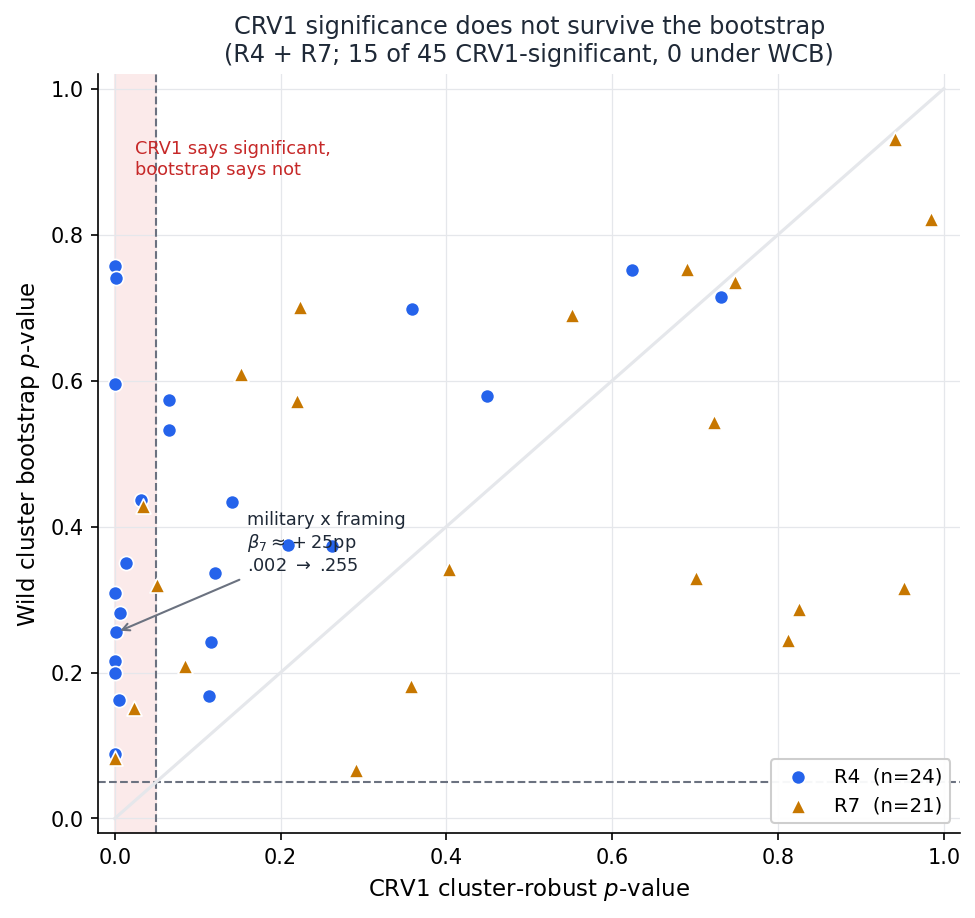
\includegraphics[width=0.72\linewidth]{figures/r4r7_crv1_vs_wcb.png}
  \caption{The CRV1-to-bootstrap collapse across both causal designs. Each point
  is one difference-in-differences estimate from R4 (per-event $\beta_3$ and
  crisis-type $\beta_7$) or R7 (per-event and pooled $\beta_3$); axes are its
  cluster-robust (CRV1) and wild-cluster-bootstrap $p$-values. Of 45 estimates,
  15 are CRV1-significant and \emph{none} survive the bootstrap: every point in
  the shaded CRV1-significant column sits above the $0.05$ line, and no point
  falls below the diagonal. The headline candidate --- military crises moving
  stake-holding communities toward security-and-military framing by
  $\beta_7\approx+25$pp --- moves from $p=0.002$ to $0.255$.}
  \label{fig:crv1-wcb}
\end{figure}

% =========================================================================
% OLD BULLET SPECIFICATION (commented out per Mohit: comment old, add new).
% Superseded by the prose above. Kept for traceability of the source numbers.
% Note: old spec said "R7: 0 of 7 cells" for the MDE; the analysis log gives
% 0 of 21 (ratios 0.04-0.47), corrected in the prose.
% =========================================================================
% \begin{description}
% \item[Setup.] Two independent causal designs: R4 (community-intensity DiD + crisis-type DDD)
%   and R7 (minority x acute DiD with subreddit and author FE).
% \item[R4 result.] CRV1 flags 9/18 per-event beta3 and 3/6 DDD beta7; WCB erases all
%   (0/18, 0/6, 0/8 on continuous Perspective toxicity). beta7 ~ +25pp moves p=0.002 -> WCB 0.255.
% \item[R7 result.] Pooled beta3 on log length -0.029 (CRV1 p=0.403, WCB p=0.342);
%   neutral sentiment p=0.023 -> WCB 0.151; 0 of 18 per-event survive.
% \item[The stronger point.] Parallel trends fail (R4: only Article 370 passes;
%   R7: all three, Wald chi2 48.8/31.3/21.7). Uninformative, not underpowered.
% \item[Why, structurally.] Crises cluster in time; each military pre-period is the
%   prior crisis aftermath. Structural confounder for crisis-response DiD.
% \item[Power.] R4 median MDE ~18pp, 0/18 detectable. R7: 0 of 7 [corrected: 0 of 21],
%   |beta3|/MDE 0.09-0.35 [corrected: 0.04-0.47].
% \item[Additional honesty.] WCB near validity floor at 7-9 clusters; over-conservative.
% \item[Descriptive residue.] R7: minority acute-phase commenters terser but less neutral.
% \item[Figures.] r7\_eventstudy\_logwords.png, r7\_mde.png, r4\_binned\_es\_secmil.png,
%   r4\_mde.png; Figure 8 = CRV1 vs WCB p-value scatter over 42 estimates.
% \item[Status.] Negative / methodological.
% \end{description}